% Created by tikzDevice version 0.12.5 on 2024-01-22 11:37:18
% !TEX encoding = UTF-8 Unicode
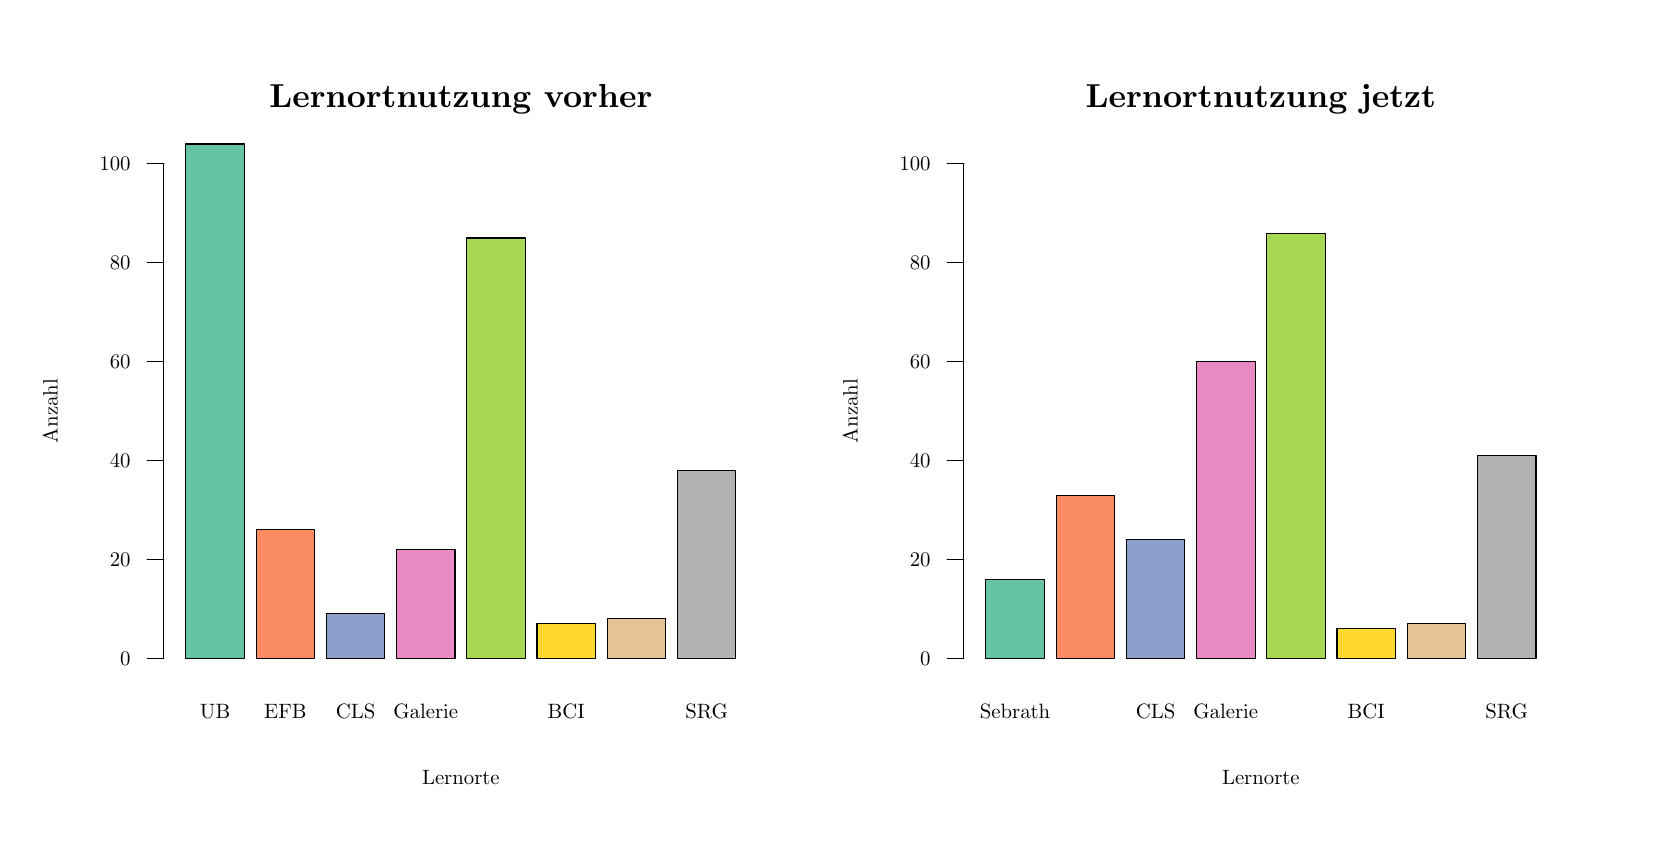
\begin{tikzpicture}[x=1pt,y=1pt]
\definecolor{fillColor}{RGB}{255,255,255}
\path[use as bounding box,fill=fillColor,fill opacity=0.00] (0,0) rectangle (578.16,289.08);
\begin{scope}
\path[clip] (  0.00,  0.00) rectangle (289.08,289.08);
\definecolor{drawColor}{RGB}{0,0,0}
\definecolor{fillColor}{RGB}{102,194,165}

\path[draw=drawColor,line width= 0.4pt,line join=round,line cap=round,fill=fillColor] ( 57.15, 61.20) rectangle ( 78.30,247.03);
\definecolor{fillColor}{RGB}{252,141,98}

\path[draw=drawColor,line width= 0.4pt,line join=round,line cap=round,fill=fillColor] ( 82.53, 61.20) rectangle (103.67,107.66);
\definecolor{fillColor}{RGB}{141,160,203}

\path[draw=drawColor,line width= 0.4pt,line join=round,line cap=round,fill=fillColor] (107.90, 61.20) rectangle (129.05, 77.28);
\definecolor{fillColor}{RGB}{231,138,195}

\path[draw=drawColor,line width= 0.4pt,line join=round,line cap=round,fill=fillColor] (133.28, 61.20) rectangle (154.43,100.51);
\definecolor{fillColor}{RGB}{166,216,84}

\path[draw=drawColor,line width= 0.4pt,line join=round,line cap=round,fill=fillColor] (158.65, 61.20) rectangle (179.80,213.08);
\definecolor{fillColor}{RGB}{255,217,47}

\path[draw=drawColor,line width= 0.4pt,line join=round,line cap=round,fill=fillColor] (184.03, 61.20) rectangle (205.18, 73.71);
\definecolor{fillColor}{RGB}{229,196,148}

\path[draw=drawColor,line width= 0.4pt,line join=round,line cap=round,fill=fillColor] (209.41, 61.20) rectangle (230.55, 75.49);
\definecolor{fillColor}{gray}{0.70}

\path[draw=drawColor,line width= 0.4pt,line join=round,line cap=round,fill=fillColor] (234.78, 61.20) rectangle (255.93,129.10);
\end{scope}
\begin{scope}
\path[clip] (  0.00,  0.00) rectangle (578.16,289.08);
\definecolor{drawColor}{RGB}{0,0,0}

\node[text=drawColor,anchor=base,inner sep=0pt, outer sep=0pt, scale=  0.75] at ( 67.72, 39.60) {UB};

\node[text=drawColor,anchor=base,inner sep=0pt, outer sep=0pt, scale=  0.75] at ( 93.10, 39.60) {EFB};

\node[text=drawColor,anchor=base,inner sep=0pt, outer sep=0pt, scale=  0.75] at (118.48, 39.60) {CLS};

\node[text=drawColor,anchor=base,inner sep=0pt, outer sep=0pt, scale=  0.75] at (143.85, 39.60) {Galerie};

\node[text=drawColor,anchor=base,inner sep=0pt, outer sep=0pt, scale=  0.75] at (194.60, 39.60) {BCI};

\node[text=drawColor,anchor=base,inner sep=0pt, outer sep=0pt, scale=  0.75] at (245.36, 39.60) {SRG};
\end{scope}
\begin{scope}
\path[clip] (  0.00,  0.00) rectangle (289.08,289.08);
\definecolor{drawColor}{RGB}{0,0,0}

\node[text=drawColor,anchor=base,inner sep=0pt, outer sep=0pt, scale=  1.20] at (156.54,260.34) {\bfseries Lernortnutzung vorher};

\node[text=drawColor,anchor=base,inner sep=0pt, outer sep=0pt, scale=  0.75] at (156.54, 15.60) {Lernorte};

\node[text=drawColor,rotate= 90.00,anchor=base,inner sep=0pt, outer sep=0pt, scale=  0.75] at ( 10.80,150.54) {Anzahl};
\end{scope}
\begin{scope}
\path[clip] (  0.00,  0.00) rectangle (578.16,289.08);
\definecolor{drawColor}{RGB}{0,0,0}

\path[draw=drawColor,line width= 0.4pt,line join=round,line cap=round] ( 49.20, 61.20) -- ( 49.20,239.88);

\path[draw=drawColor,line width= 0.4pt,line join=round,line cap=round] ( 49.20, 61.20) -- ( 43.20, 61.20);

\path[draw=drawColor,line width= 0.4pt,line join=round,line cap=round] ( 49.20, 96.94) -- ( 43.20, 96.94);

\path[draw=drawColor,line width= 0.4pt,line join=round,line cap=round] ( 49.20,132.67) -- ( 43.20,132.67);

\path[draw=drawColor,line width= 0.4pt,line join=round,line cap=round] ( 49.20,168.41) -- ( 43.20,168.41);

\path[draw=drawColor,line width= 0.4pt,line join=round,line cap=round] ( 49.20,204.14) -- ( 43.20,204.14);

\path[draw=drawColor,line width= 0.4pt,line join=round,line cap=round] ( 49.20,239.88) -- ( 43.20,239.88);

\node[text=drawColor,anchor=base east,inner sep=0pt, outer sep=0pt, scale=  0.75] at ( 37.20, 58.62) {0};

\node[text=drawColor,anchor=base east,inner sep=0pt, outer sep=0pt, scale=  0.75] at ( 37.20, 94.35) {20};

\node[text=drawColor,anchor=base east,inner sep=0pt, outer sep=0pt, scale=  0.75] at ( 37.20,130.09) {40};

\node[text=drawColor,anchor=base east,inner sep=0pt, outer sep=0pt, scale=  0.75] at ( 37.20,165.83) {60};

\node[text=drawColor,anchor=base east,inner sep=0pt, outer sep=0pt, scale=  0.75] at ( 37.20,201.56) {80};

\node[text=drawColor,anchor=base east,inner sep=0pt, outer sep=0pt, scale=  0.75] at ( 37.20,237.30) {100};
\end{scope}
\begin{scope}
\path[clip] (289.08,  0.00) rectangle (578.16,289.08);
\definecolor{drawColor}{RGB}{0,0,0}
\definecolor{fillColor}{RGB}{102,194,165}

\path[draw=drawColor,line width= 0.4pt,line join=round,line cap=round,fill=fillColor] (346.23, 61.20) rectangle (367.38, 89.79);
\definecolor{fillColor}{RGB}{252,141,98}

\path[draw=drawColor,line width= 0.4pt,line join=round,line cap=round,fill=fillColor] (371.61, 61.20) rectangle (392.75,120.16);
\definecolor{fillColor}{RGB}{141,160,203}

\path[draw=drawColor,line width= 0.4pt,line join=round,line cap=round,fill=fillColor] (396.98, 61.20) rectangle (418.13,104.08);
\definecolor{fillColor}{RGB}{231,138,195}

\path[draw=drawColor,line width= 0.4pt,line join=round,line cap=round,fill=fillColor] (422.36, 61.20) rectangle (443.51,168.41);
\definecolor{fillColor}{RGB}{166,216,84}

\path[draw=drawColor,line width= 0.4pt,line join=round,line cap=round,fill=fillColor] (447.73, 61.20) rectangle (468.88,214.86);
\definecolor{fillColor}{RGB}{255,217,47}

\path[draw=drawColor,line width= 0.4pt,line join=round,line cap=round,fill=fillColor] (473.11, 61.20) rectangle (494.26, 71.92);
\definecolor{fillColor}{RGB}{229,196,148}

\path[draw=drawColor,line width= 0.4pt,line join=round,line cap=round,fill=fillColor] (498.49, 61.20) rectangle (519.63, 73.71);
\definecolor{fillColor}{gray}{0.70}

\path[draw=drawColor,line width= 0.4pt,line join=round,line cap=round,fill=fillColor] (523.86, 61.20) rectangle (545.01,134.46);
\end{scope}
\begin{scope}
\path[clip] (  0.00,  0.00) rectangle (578.16,289.08);
\definecolor{drawColor}{RGB}{0,0,0}

\node[text=drawColor,anchor=base,inner sep=0pt, outer sep=0pt, scale=  0.75] at (356.80, 39.60) {Sebrath};

\node[text=drawColor,anchor=base,inner sep=0pt, outer sep=0pt, scale=  0.75] at (407.56, 39.60) {CLS};

\node[text=drawColor,anchor=base,inner sep=0pt, outer sep=0pt, scale=  0.75] at (432.93, 39.60) {Galerie};

\node[text=drawColor,anchor=base,inner sep=0pt, outer sep=0pt, scale=  0.75] at (483.68, 39.60) {BCI};

\node[text=drawColor,anchor=base,inner sep=0pt, outer sep=0pt, scale=  0.75] at (534.44, 39.60) {SRG};
\end{scope}
\begin{scope}
\path[clip] (289.08,  0.00) rectangle (578.16,289.08);
\definecolor{drawColor}{RGB}{0,0,0}

\node[text=drawColor,anchor=base,inner sep=0pt, outer sep=0pt, scale=  1.20] at (445.62,260.34) {\bfseries Lernortnutzung jetzt};

\node[text=drawColor,anchor=base,inner sep=0pt, outer sep=0pt, scale=  0.75] at (445.62, 15.60) {Lernorte};

\node[text=drawColor,rotate= 90.00,anchor=base,inner sep=0pt, outer sep=0pt, scale=  0.75] at (299.88,150.54) {Anzahl};
\end{scope}
\begin{scope}
\path[clip] (  0.00,  0.00) rectangle (578.16,289.08);
\definecolor{drawColor}{RGB}{0,0,0}

\path[draw=drawColor,line width= 0.4pt,line join=round,line cap=round] (338.28, 61.20) -- (338.28,239.88);

\path[draw=drawColor,line width= 0.4pt,line join=round,line cap=round] (338.28, 61.20) -- (332.28, 61.20);

\path[draw=drawColor,line width= 0.4pt,line join=round,line cap=round] (338.28, 96.94) -- (332.28, 96.94);

\path[draw=drawColor,line width= 0.4pt,line join=round,line cap=round] (338.28,132.67) -- (332.28,132.67);

\path[draw=drawColor,line width= 0.4pt,line join=round,line cap=round] (338.28,168.41) -- (332.28,168.41);

\path[draw=drawColor,line width= 0.4pt,line join=round,line cap=round] (338.28,204.14) -- (332.28,204.14);

\path[draw=drawColor,line width= 0.4pt,line join=round,line cap=round] (338.28,239.88) -- (332.28,239.88);

\node[text=drawColor,anchor=base east,inner sep=0pt, outer sep=0pt, scale=  0.75] at (326.28, 58.62) {0};

\node[text=drawColor,anchor=base east,inner sep=0pt, outer sep=0pt, scale=  0.75] at (326.28, 94.35) {20};

\node[text=drawColor,anchor=base east,inner sep=0pt, outer sep=0pt, scale=  0.75] at (326.28,130.09) {40};

\node[text=drawColor,anchor=base east,inner sep=0pt, outer sep=0pt, scale=  0.75] at (326.28,165.83) {60};

\node[text=drawColor,anchor=base east,inner sep=0pt, outer sep=0pt, scale=  0.75] at (326.28,201.56) {80};

\node[text=drawColor,anchor=base east,inner sep=0pt, outer sep=0pt, scale=  0.75] at (326.28,237.30) {100};
\end{scope}
\end{tikzpicture}
